% Options for packages loaded elsewhere
\PassOptionsToPackage{unicode}{hyperref}
\PassOptionsToPackage{hyphens}{url}
%
\documentclass[
  ignorenonframetext,
  serif,
  professionalfont,
  usenames,
  dvipsnames,
  aspectratio = 169]{beamer}
\usepackage{pgfpages}
\setbeamertemplate{caption}[numbered]
\setbeamertemplate{caption label separator}{: }
\setbeamercolor{caption name}{fg=normal text.fg}
\beamertemplatenavigationsymbolsempty
% Prevent slide breaks in the middle of a paragraph
\widowpenalties 1 10000
\raggedbottom
\setbeamertemplate{part page}{
  \centering
  \begin{beamercolorbox}[sep=16pt,center]{part title}
    \usebeamerfont{part title}\insertpart\par
  \end{beamercolorbox}
}
\setbeamertemplate{section page}{
  \centering
  \begin{beamercolorbox}[sep=12pt,center]{section title}
    \usebeamerfont{section title}\insertsection\par
  \end{beamercolorbox}
}
\setbeamertemplate{subsection page}{
  \centering
  \begin{beamercolorbox}[sep=8pt,center]{subsection title}
    \usebeamerfont{subsection title}\insertsubsection\par
  \end{beamercolorbox}
}
\AtBeginPart{
  \frame{\partpage}
}
\AtBeginSection{
  \ifbibliography
  \else
    \frame{\sectionpage}
  \fi
}
\AtBeginSubsection{
  \frame{\subsectionpage}
}
\usepackage{amsmath,amssymb}
\usepackage{iftex}
\ifPDFTeX
  \usepackage[T1]{fontenc}
  \usepackage[utf8]{inputenc}
  \usepackage{textcomp} % provide euro and other symbols
\else % if luatex or xetex
  \usepackage{unicode-math} % this also loads fontspec
  \defaultfontfeatures{Scale=MatchLowercase}
  \defaultfontfeatures[\rmfamily]{Ligatures=TeX,Scale=1}
\fi
\usepackage{lmodern}
\ifPDFTeX\else
  % xetex/luatex font selection
\fi
% Use upquote if available, for straight quotes in verbatim environments
\IfFileExists{upquote.sty}{\usepackage{upquote}}{}
\IfFileExists{microtype.sty}{% use microtype if available
  \usepackage[]{microtype}
  \UseMicrotypeSet[protrusion]{basicmath} % disable protrusion for tt fonts
}{}
\makeatletter
\@ifundefined{KOMAClassName}{% if non-KOMA class
  \IfFileExists{parskip.sty}{%
    \usepackage{parskip}
  }{% else
    \setlength{\parindent}{0pt}
    \setlength{\parskip}{6pt plus 2pt minus 1pt}}
}{% if KOMA class
  \KOMAoptions{parskip=half}}
\makeatother
\usepackage{xcolor}
\newif\ifbibliography
\usepackage{longtable,booktabs,array}
\usepackage{calc} % for calculating minipage widths
\usepackage{caption}
% Make caption package work with longtable
\makeatletter
\def\fnum@table{\tablename~\thetable}
\makeatother
\usepackage{graphicx}
\makeatletter
\newsavebox\pandoc@box
\newcommand*\pandocbounded[1]{% scales image to fit in text height/width
  \sbox\pandoc@box{#1}%
  \Gscale@div\@tempa{\textheight}{\dimexpr\ht\pandoc@box+\dp\pandoc@box\relax}%
  \Gscale@div\@tempb{\linewidth}{\wd\pandoc@box}%
  \ifdim\@tempb\p@<\@tempa\p@\let\@tempa\@tempb\fi% select the smaller of both
  \ifdim\@tempa\p@<\p@\scalebox{\@tempa}{\usebox\pandoc@box}%
  \else\usebox{\pandoc@box}%
  \fi%
}
% Set default figure placement to htbp
\def\fps@figure{htbp}
\makeatother
\setlength{\emergencystretch}{3em} % prevent overfull lines
\providecommand{\tightlist}{%
  \setlength{\itemsep}{0pt}\setlength{\parskip}{0pt}}
\setcounter{secnumdepth}{-\maxdimen} % remove section numbering
% Definição do esquema de cores:
% 1. UFPR - Azul com cinza.
% 2. DEST - Roxo com cinza.
% 3. LEG - Laranjado com cinza.
\def\mycolorscheme{1}

% Caminho para a imagem de fundo com aspecto 16x9.
% \def\pathtobg{config/ufpr-fachada-baixo-1.jpg}
% \def\pathtobg{config/ufpr-fundo.jpg}
% \def\pathtobg{config/ufpr-fundo.jpg}
\def\pathtobg{./config/ufpr-fundo-16x9.jpg}

% \providecommand{\tightlist}{%
%   \setlength{\itemsep}{0pt}\setlength{\parskip}{0pt}}
% ATTENTION: Redefine o comando acima que é definido pelo template.
% \renewcommand{\tightlist}{}
\renewcommand{\tightlist}{%
  \setlength{\itemsep}{0\baselineskip}
  \setlength{\parskip}{0.25\baselineskip}
}

% Logo na capa.
\titlegraphic{
  %\vspace{-1em}
  %
\includegraphics[height=1.2cm]{config/dest-texto-2.png}\hspace{1em}
  %\includegraphics[height=1.8cm]{config/dsbd-logo-2x2.png}\hspace{1em}
  
\includegraphics[height=1.8cm]{config/ufpr-transparent-600px.png}
}
%-----------------------------------------------------------------------

% Palladio.
% \usepackage[sc]{mathpazo}
% \linespread{1.05}         % Palladio needs more leading (space between lines)
% \usepackage[T1]{fontenc}

% Kurier.
% \usepackage[light, condensed, math]{kurier}
% \usepackage[T1]{fontenc}

% Iwona.
% \usepackage[math, light, condensed]{iwona}

% \usepackage{cmbright}
% \usepackage[charter]{mathdesign}
% \usepackage{palatino}

% Roboto (with Iwona for maths).
% \usepackage[math]{iwona}
% \usepackage[sfdefault, light, condensed]{roboto}

% Source Sans Pro (with Iwona for maths).
% \usepackage[math]{iwona}
% \usepackage[default, light]{sourcesanspro}

% Lato (with Iwona for maths).
% \usepackage[math]{iwona}
% \usepackage[default]{lato}

% Fira Sans (with Iwona for maths).
\usepackage[math, light]{iwona}
\usepackage[sfdefault,light]{FiraSans} %% option 'sfdefault' activates Fira Sans as the default text font
\usepackage[T1]{fontenc}
\renewcommand*\oldstylenums[1]{{\firaoldstyle #1}}

% Font for code. ----------------------------
% \usepackage[scaled=.75]{beramono}
\usepackage{inconsolata}

% ATTENTION: needs complile with xelatex: `$ xelatex file.tex`
% \usepackage{fontspec}
% \setmonofont{M+ 1m}
% \setmonofont{M+ 1mn}
% \setmonofont{M+ 2m}

%-----------------------------------------------------------------------

% \usepackage{lmodern}
\usepackage{amssymb, amsmath}
\usepackage[makeroom]{cancel}
% \usepackage{ifxetex, ifluatex}
\usepackage{fixltx2e} % provides \textsubscript
\usepackage[utf8]{inputenc}
\usepackage[shorthands=off,main=brazil]{babel}
\usepackage{graphicx}
\usepackage{xcolor}
\usepackage{setspace}
\usepackage{comment}
\usepackage{icomma}

%-----------------------------------------------------------------------
% Algumas configurações.

\setlength{\parindent}{0pt}
\setlength{\parskip}{6pt plus 2pt minus 1pt}
\setlength{\emergencystretch}{3em}  % prevent overfull lines
% \providecommand{\tightlist}{%
%   \setlength{\itemsep}{0pt}\setlength{\parskip}{0pt}}
\setcounter{secnumdepth}{0}

% Espaço vertical para o ambiente `quote`.
\let\oldquote\quote
\let\oldendquote\endquote
\renewenvironment{quote}{%
  \vspace{1em}\oldquote}{%
  \oldendquote\vspace{1em}}

%-----------------------------------------------------------------------
% Espaçamento entre items para itemize, enumerate e description.

% % itemize.
% \let\itemopen\itemize
% \let\itemclose\enditemize
% \renewenvironment{itemize}{%
%   \itemopen\addtolength{\itemsep}{0.25\baselineskip}}{\itemclose}
%
% % enumerate.
% \let\enumopen\enumerate
% \let\enumclose\endenumerate
% \renewenvironment{enumerate}{%
%   \enumopen\addtolength{\itemsep}{0.25\baselineskip}}{\enumclose}
%
% % description.
% \let\descopen\description
% \let\descclose\enddescription
% \renewenvironment{description}{%
%   \descopen\addtolength{\itemsep}{0.25\baselineskip}}{\descclose}

%-----------------------------------------------------------------------

% \usepackage[hang]{caption}
\usepackage{caption}
\captionsetup{font=footnotesize,
  labelfont={color=mycolor1, footnotesize},
  labelsep=period}

% \providecommand{\tightlist}{%
%   \setlength{\itemsep}{0pt}\setlength{\parskip}{0pt}}

%-----------------------------------------------------------------------

\usepackage{tikz}

% \def\pathtobg{/home/walmes/Projects/templates/COMMON/ufpr-fundo.jpg}
% \def\pathtobg{/home/walmes/Projects/templates/COMMON/ufpr-fundo-16x9.jpg}
% \def\pathtobg{/home/walmes/Projects/templates/COMMON/ufpr-fachada-dir-1.jpg}
% \def\pathtobg{/home/walmes/Projects/templates/COMMON/ufpr-fachada-esq-1.jpg}
% \def\pathtobg{/home/walmes/Projects/templates/COMMON/ufpr-perto-1.jpg}
% \def\pathtobg{/home/walmes/Projects/templates/COMMON/ufpr-fachada-baixo-1.jpg}

\ifx\pathtobg\undefined
\else
  \usebackgroundtemplate{
    \tikz[overlay, remember picture]
    \node[% opacity=0.3,
          at=(current page.south east),
          anchor=south east,
          inner sep=0pt] {
            \includegraphics[height=\paperheight, width=\paperwidth]{\pathtobg}};
  }
\fi

%-----------------------------------------------------------------------
% Definições de esquema de cores.

\ifx\mycolorscheme\undefined
  % UFPR.
  % http://www.color-hex.com/color-palette/2018
  \definecolor{mycolor1}{HTML}{015c93} % Título.
  \definecolor{mycolor2}{HTML}{363435} % Texto.
  \definecolor{mycolor3}{HTML}{015c93} % Estrutura.
  \definecolor{mycolor4}{HTML}{015c93} % Links.
  \definecolor{mycolor5}{HTML}{CECAC5} % Preenchimentos.
\else
  \if\mycolorscheme1
    % UFPR.
    \definecolor{mycolor1}{HTML}{015c93} % Título.
    \definecolor{mycolor2}{HTML}{363435} % Texto.
    \definecolor{mycolor3}{HTML}{015c93} % Estrutura.
    \definecolor{mycolor4}{HTML}{015c93} % Links.
    \definecolor{mycolor5}{HTML}{CECAC5} % Preenchimentos.
  \fi
  \if\mycolorscheme2
    % DEST.
    \definecolor{mycolor1}{HTML}{2a0e72} % Título.
    \definecolor{mycolor2}{HTML}{202E35} % Texto.
    \definecolor{mycolor3}{HTML}{2a0e72} % Estrutura.
    % \definecolor{mycolor3}{HTML}{8072a3} % Estrutura.
    \definecolor{mycolor4}{HTML}{2a0e72} % Links.
    % \definecolor{mycolor4}{HTML}{bfb9d1} % Links.
    % \definecolor{mycolor5}{HTML}{AEA79F} % Preenchimentos.
    \definecolor{mycolor5}{HTML}{CECAC5} % Preenchimentos.
  \fi
  \if\mycolorscheme3
    % LEG.
    \definecolor{mycolor2}{HTML}{363435} % Texto.
    % \definecolor{mycolor1}{HTML}{ff8000} % Título.
    % \definecolor{mycolor3}{HTML}{ff8000} % Estrutura.
    % \definecolor{mycolor4}{HTML}{ff8000} % Links.
    % \definecolor{mycolor1}{HTML}{E57300} % Título.
    % \definecolor{mycolor3}{HTML}{E57300} % Estrutura.
    % \definecolor{mycolor4}{HTML}{E57300} % Links.
    \definecolor{mycolor1}{HTML}{F67014} % Título.
    \definecolor{mycolor3}{HTML}{F67014} % Estrutura.
    \definecolor{mycolor4}{HTML}{F67014} % Links.
    % \definecolor{mycolor1}{HTML}{FE5C23} % Título.
    % \definecolor{mycolor3}{HTML}{FE5C23} % Estrutura.
    % \definecolor{mycolor4}{HTML}{FE5C23} % Links.
    \definecolor{mycolor5}{HTML}{222222} % Preenchimentos.
    \definecolor{mycolor5}{HTML}{383838} % Preenchimentos.
  \fi
\fi

\hypersetup{
  colorlinks=true,
  linkcolor=mycolor4,
  urlcolor=mycolor1,
  citecolor=mycolor1
}

%-----------------------------------------------------------------------
% ATTENTION: http://www.cpt.univ-mrs.fr/~masson/latex/Beamer-appearance-cheat-sheet.pdf

\usetheme{Boadilla}
\usecolortheme{default}

% \setbeamersize{text margin left=7mm, text margin right=7mm}
% \setbeamertemplate{frametitle}[default][left, leftskip=3mm]
% \addtobeamertemplate{frametitle}{\vspace{0.5em}}{}

\setbeamertemplate{caption}[numbered]
\setbeamertemplate{section in toc}[sections numbered]
\setbeamertemplate{subsection in toc}[subsections numbered]
\setbeamertemplate{sections/subsections in toc}[ball]{}
\setbeamertemplate{sections in toc}[ball]
\setbeamercolor{section number projected}{bg=mycolor1, fg=white}
\setbeamertemplate{blocks}[rounded]
\setbeamertemplate{navigation symbols}{}
\setbeamertemplate{frametitle continuation}{\gdef\beamer@frametitle{}}
% \setbeamertemplate{frametitle}[default][center]
% \setbeamertemplate{footline}[frame number]

\setbeamertemplate{enumerate items}[default]
\setbeamertemplate{itemize items}{\scriptsize\raise1.25pt\hbox{\donotcoloroutermaths$\blacktriangleright$}}

% Blocos.
% \addtobeamertemplate{block begin}{\vskip -\bigskipamount}{}
% \addtobeamertemplate{block end}{}{\vskip -\bigskipamount}
\addtobeamertemplate{block begin}{\vspace{0.5em}}{}
\addtobeamertemplate{block end}{}{\vspace{0.5em}}


% Rodapé.
\setbeamercolor{title in head/foot}{parent=subsection in head/foot}
\setbeamercolor{author in head/foot}{bg=mycolor4, fg=white}
\setbeamercolor{date in head/foot}{parent=subsection in head/foot, fg=mycolor3}

% Cabeçalho.
\setbeamercolor{section in head/foot}{bg=mycolor2, fg=mycolor4}
\setbeamercolor{subsection in head/foot}{bg=mycolor2, fg=white}

\setbeamercolor{title}{fg=mycolor1}       % Título dos slides.
\setbeamercolor{titlelike}{fg=title}
\setbeamercolor{subtitle}{fg=mycolor2}    % Subtítulo.
\setbeamercolor{institute in head/foot}{parent=palette primary} % Instituição.
\setbeamercolor{frametitle}{fg=mycolor1}  % De quadro.
\setbeamercolor{structure}{fg=mycolor3}   % Listas e rodapé.
\setbeamercolor{item projected}{bg=mycolor2}
\setbeamercolor{block title}{bg=mycolor5, fg=mycolor2}
\setbeamercolor{normal text}{fg=mycolor2} % Texto.
\setbeamercolor{caption name}{fg=normal text.fg}
% \setbeamercolor{footlinecolor}{fg=mycolor2, bg=mycolor5}
% \setbeamercolor{section in head/foot}{fg=mycolor2, bg=mycolor5}
\setbeamercolor{author in head/foot}{fg=white, bg=mycolor1}
\setbeamercolor{section in foot}{fg=mycolor4, bg=mycolor5}
\setbeamercolor{date in foot}{fg=mycolor4, bg=mycolor5}
\setbeamercolor{block title}{fg=white, bg=mycolor1}
\setbeamercolor{block body}{fg=black, bg=white!80!gray}
\setbeamercolor{block body}{fg=black, bg=white!80!gray}

% To remove empty brackets of \institution.
\makeatletter
\setbeamertemplate{footline}{
  \leavevmode%
  \hbox{%
    \begin{beamercolorbox}[
      wd=0.3\paperwidth, ht=2.25ex, dp=1ex, right]{author in head/foot}%
      \usebeamerfont{author in head/foot}\insertshortauthor{}\hspace*{1ex}
    \end{beamercolorbox}%
    \begin{beamercolorbox}[
      wd=0.6\paperwidth, ht=2.25ex, dp=1ex, left]{section in foot}%
      \usebeamerfont{title in head/foot}\hspace*{1ex}\insertshorttitle{}
      % \usebeamerfont{title in head/foot}\hspace*{1ex}\insertframetitle{}
    \end{beamercolorbox}%
    \begin{beamercolorbox}[
      wd=0.1\paperwidth, ht=2.25ex, dp=1ex, right]{date in foot}%
      \insertframenumber{}\hspace*{2ex}
    \end{beamercolorbox}
  }%
  \vskip0pt%
}
\makeatother

%-----------------------------------------------------------------------

% \usepackage{hyphenat}
\usepackage{changepage}

% Slide para o título das seções.
\AtBeginSection[]{
  \begin{frame}
    % \vfill
    \vspace{4cm}
    % \centering
    % \begin{beamercolorbox}[sep = 8pt, center, shadow = true, rounded = true]{title}
    \begin{beamercolorbox}{title}
      \begin{columns}
        \column{0.7\linewidth}
        {\LARGE\textbf \insertsectionhead}
      \end{columns}
    \end{beamercolorbox}
    \vfill
  \end{frame}
}

%-----------------------------------------------------------------------
%---- preamble-chunk.tex -----------------------------------------------

% Knitr.

% ATTENTION: this needs `\usepackage{xcolor}'.
\definecolor{color_line}{HTML}{333333}
\definecolor{color_back}{HTML}{DDDDDD}
% \definecolor{color_back}{HTML}{FF0000}

% ATTENTION: usa o fancyvrb.
% https://ctan.math.illinois.edu/macros/latex/contrib/fancyvrb/doc/fancyvrb-doc.pdf
% R input.
\usepackage{tcolorbox}
\ifcsmacro{Highlighting}{
  % Statment if it exists. ------------------
  \DefineVerbatimEnvironment{Highlighting}{Verbatim}{
    % frame=lines,     % Linha superior e inferior.
    % framerule=0.5pt, % Espessura da linha.
    framesep=2ex,    % Distância da linha para o texto.
    % rulecolor=\color{color_line},
    % numbers=right,
    fontsize=\footnotesize, % Tamanho da fonte.
    baselinestretch=0.8,    % Espaçamento entre linhas.
    commandchars=\\\{\}}
  % Margens do ambiente `Shaded'.
  % \fvset{listparameters={\setlength{\topsep}{-1em}}}
  % \renewenvironment{Shaded}{\vspace{-1ex}}{\vspace{-2ex}}
  \renewenvironment{Shaded}{
    \vspace{2pt}
    \begin{tcolorbox}[
      boxrule=0pt,      % Espessura do contorno.
      colframe=gray!10, % Cor do contorno.
      colback=gray!10,  % Cor de fundo da caixa.
      arc=1em,          % Raio para contornos arredondados.
      sharp corners,
      boxsep=0.5em,     % Margem interna.
      left=3pt, right=3pt, top=3pt, bottom=3pt, % Margens internas.
      grow to left by=0mm,
      grow to right by=6pt,
      ]
    }{
    \end{tcolorbox}
    \vspace{-3pt}
    }
  }{
  % Statment if it not exists. --------------
}

% R output e todo `verbatim'.
\makeatletter
\def\verbatim@font{\linespread{0.8}\ttfamily\footnotesize}
%\makeatother

% Cor de fundo e margens do `verbatim'.
\let\oldv\verbatim
\let\oldendv\endverbatim

\def\verbatim{%
  \par\setbox0\vbox\bgroup % Abre grupo.
  %\vspace{-5px}            % Reduz margem superior.
  \oldv                    % Chama abertura do verbatim.
}
\def\endverbatim{%
  \oldendv                 % Chama encerramento do verbatim.
  %\vspace{0cm}           % Controla margem inferior.
  \egroup%\fboxsep5px      % Fecha grupo.
  \noindent{{\usebox0}}\par
}

%-----------------------------------------------------------------------
%---- preamble-commands.tex --------------------------------------------

% Para fazer texto em duas colunas.
\newcommand{\mytwocolumns}[4]{
  % #1: Line width fraction for the left column , e.g. 0.5.
  % #2: Line width fraction for the right column.
  % #3: Content for the left column.
  % #4: Content for the right column.
  \begin{columns}[c]
    \begin{column}{#1\linewidth} %----------- left.
      #3
    \end{column} %--------------------------- left.
    \begin{column}{#2\linewidth} %----------- right.
      #4
    \end{column} %--------------------------- right.
  \end{columns}
}

%-----------------------------------------------------------------------
% Para fazer duas colunas no Rmd.

% Center vertical align.
\def\beginAHalfColumn{\begin{minipage}{0.49\textwidth}}%
\def\beginAlmostHalfColumn{\begin{minipage}{0.45\textwidth}}%
\def\beginAQuarterColumn{\begin{minipage}{0.23\textwidth}}%
\def\beginThreeQuartersColumn{\begin{minipage}{0.72\textwidth}}%
\def\beginAThirdColumn{\begin{minipage}{0.31\textwidth}}%
\def\beginTwoThirdsColumn{\begin{minipage}{0.64\textwidth}}%
\def\endColumns{\end{minipage}}%

% Top vertical align.
\def\beginAHalfColumnT{\begin{minipage}[t]{0.49\textwidth}}%
\def\beginAlmostHalfColumnT{\begin{minipage}[t]{0.45\textwidth}}%
\def\beginAQuarterColumnT{\begin{minipage}[t]{0.23\textwidth}}%
\def\beginThreeQuartersColumnT{\begin{minipage}[t]{0.72\textwidth}}%
\def\beginAThirdColumnT{\begin{minipage}[t]{0.31\textwidth}}%
\def\beginTwoThirdsColumnT{\begin{minipage}[t]{0.64\textwidth}}%

%---------------------------------------------------------------------
% Ambientes para frases como e sem imagem.

\newcommand{\myquote}[3]{
  % #1: caminho para a imagem.
  % #2: a frase/quotation.
  % #3: o autor.
  \begin{center}
    \begin{minipage}[c]{0.19\linewidth}
      \begin{center}
        \includegraphics[height=2.5cm]{#1}
      \end{center}
    \end{minipage}
    \begin{minipage}[c]{0.7\linewidth}
      \begin{flushright}
        \textit{#2}
        \vspace{1ex}

        -- #3
      \end{flushright}
    \end{minipage}
  \end{center}
}

\newcommand{\myphrase}[2]{
  % #1: a frase/quotation.
  % #2: o autor.
  \begin{center}
    \begin{minipage}[c]{0.19\linewidth}
    \end{minipage}
    \begin{minipage}[c]{0.7\linewidth}
      \begin{flushright}
        \textit{#1}
        \vspace{1ex}

        -- #2
      \end{flushright}
    \end{minipage}
  \end{center}
}

%-----------------------------------------------------------------------
% Comandos para texto em destaque.

% \newcommand{\hi}[1]{%
%   \textcolor{ubuntu_orange}{#1}\xspace
% }

\usepackage{xspace}

% URLs com letra miuda.
\newcommand{\myurl}[1]{%
  {\tiny \url{#1}}\xspace
}

% Botões.
\newcommand{\btn}[1]{%
  \beamergotobutton{#1}\xspace
}

% Texto grande centralizado.
\newcommand{\centertitle}[1]{%
  \begin{center}
    {\LARGE \bfseries \hi{#1}}
  \end{center}
}

%-----------------------------------------------------------------------
\usepackage{bookmark}
\IfFileExists{xurl.sty}{\usepackage{xurl}}{} % add URL line breaks if available
\urlstyle{same}
\hypersetup{
  pdfauthor={Prof.~Me. Lineu Alberto Cavazani de Freitas },
  hidelinks,
  pdfcreator={LaTeX via pandoc}}

\title{\hfill\break
\textbf{Fundamentos de Análise Exploratória de Dados}\\
Conceitos e Aplicações}
\subtitle{\hfill\break
Encontro 1\\
Exercícios}
\author{Prof.~Me. Lineu Alberto Cavazani de Freitas \vspace{-0.5cm}}
\date{}

\begin{document}
\frame{\titlepage}

\section{Exercício 1}\label{exercuxedcio-1}

\begin{frame}{Exercício 1}
\phantomsection\label{exercuxedcio-1-1}
Classifique cada uma das variáveis a seguir em quantitativa contínua
(QC), quantitativa discreta (QD), qualitativa nominal (QN) ou
qualitativa ordinal (QO).

\vspace{0.3cm}

\beginAHalfColumn

\begin{enumerate}
\tightlist
\item
  Estado civil.
\item
  Peso.
\item
  Número de filhos.
\item
  Número da camisa de um jogador.
\item
  Classe social.
\item
  Idade.
\item
  Classificação como doente ou não doente.
\item
  Número de animais de estimação.
\end{enumerate}

\endColumns
\beginAHalfColumn

\begin{enumerate}
\setcounter{enumi}{8}
\tightlist
\item
  Tempo.
\item
  Número de consultas médicas.
\item
  Severidade de uma lesão.
\item
  Gols marcados em um jogo.
\item
  Grau de escolaridade.
\item
  Altura.
\item
  Cor da pele.
\item
  Grau de proficiência em língua inglesa.
\end{enumerate}

\endColumns
\end{frame}

\begin{frame}{Exercício 1}
\phantomsection\label{exercuxedcio-1-2}
Classifique cada uma das variáveis a seguir em quantitativa contínua
(QC), quantitativa discreta (QD), qualitativa nominal (QN) ou
qualitativa ordinal (QO).

\vspace{0.3cm}

\beginAHalfColumn

\begin{enumerate}
\tightlist
\item
  Estado civil. (\textbf{QN})
\item
  Peso. (\textbf{QC})
\item
  Número de filhos. (\textbf{QD})
\item
  Número da camisa de um jogador. (\textbf{QN})
\item
  Classe social. (\textbf{QO})
\item
  Idade. (\textbf{QC})
\item
  Classificação como doente ou não doente. (\textbf{QN})
\item
  Número de animais de estimação. (\textbf{QD})
\end{enumerate}

\endColumns
\beginAHalfColumn

\begin{enumerate}
\setcounter{enumi}{8}
\tightlist
\item
  Tempo. (\textbf{QC})
\item
  Número de consultas médicas. (\textbf{QD})
\item
  Severidade de uma lesão. (\textbf{QO})
\item
  Gols marcados em um jogo. (\textbf{QD})
\item
  Grau de escolaridade. (\textbf{QO})
\item
  Altura. (\textbf{QC})
\item
  Cor da pele. (\textbf{QN})
\item
  Grau de proficiência em língua inglesa. (\textbf{QO})
\end{enumerate}

\endColumns
\end{frame}

\section{Exercício 2}\label{exercuxedcio-2}

\begin{frame}{Exercício 2}
\phantomsection\label{exercuxedcio-2-1}
Classifique os estudos descritos na sequência como experimentais (EE) ou
observacionais (EO).

\begin{enumerate}
\item
  Automóveis que circulam por uma rodovia foram selecionados
  inspecionados com o objetivo de analisar a emissão de poluentes.
\item
  Dois tipos de pintura foram aplicados a móveis de madeira com o
  objetivo de avaliar a aderência da tinta.
\item
  As capacidades respiratórias de funcionários fumantes e não fumantes
  foram verificadas numa pesquisa.
\item
  Numa plantação, três tipos de fertilizantes foram administrados a
  diferentes canteiros, e as consequentes produções foram registradas.
\item
  Automóveis de certo modelo foram analisados quanto ao desempenho
  registrado quando abastecidos com álcool e gasolina.
\item
  As preferências de consumidores de certo produto foram registradas
  quando apresentados a dois tipos de embalagens.
\end{enumerate}
\end{frame}

\begin{frame}{Exercício 2}
\phantomsection\label{exercuxedcio-2-2}
Classifique os estudos descritos na sequência como experimentais (EE) ou
observacionais (EO).

\begin{enumerate}
\item
  Automóveis que circulam por uma rodovia foram selecionados
  inspecionados com o objetivo de analisar a emissão de poluentes.
  (\textbf{EO})
\item
  Dois tipos de pintura foram aplicados a móveis de madeira com o
  objetivo de avaliar a aderência da tinta. (\textbf{EE})
\item
  As capacidades respiratórias de funcionários fumantes e não fumantes
  foram verificadas numa pesquisa. (\textbf{EO})
\item
  Numa plantação, três tipos de fertilizantes foram administrados a
  diferentes canteiros, e as consequentes produções foram registradas.
  (\textbf{EE})
\item
  Automóveis de certo modelo foram analisados quanto ao desempenho
  registrado quando abastecidos com álcool e gasolina. (\textbf{EE})
\item
  As preferências de consumidores de certo produto foram registradas
  quando apresentados a dois tipos de embalagens. (\textbf{EO})
\end{enumerate}
\end{frame}

\section{Exercício 3}\label{exercuxedcio-3}

\begin{frame}{Exercício 3}
\phantomsection\label{exercuxedcio-3-1}
Uma pesquisa tinha como objetivo verificar qual o meio de transporte
mais comum entre os alunos de uma turma. As respostas foram:

\begin{longtable}[]{@{}
  >{\raggedright\arraybackslash}p{(\linewidth - 20\tabcolsep) * \real{0.0411}}
  >{\raggedright\arraybackslash}p{(\linewidth - 20\tabcolsep) * \real{0.0822}}
  >{\raggedright\arraybackslash}p{(\linewidth - 20\tabcolsep) * \real{0.0959}}
  >{\raggedright\arraybackslash}p{(\linewidth - 20\tabcolsep) * \real{0.0959}}
  >{\raggedright\arraybackslash}p{(\linewidth - 20\tabcolsep) * \real{0.0959}}
  >{\raggedright\arraybackslash}p{(\linewidth - 20\tabcolsep) * \real{0.0822}}
  >{\raggedright\arraybackslash}p{(\linewidth - 20\tabcolsep) * \real{0.0959}}
  >{\raggedright\arraybackslash}p{(\linewidth - 20\tabcolsep) * \real{0.0822}}
  >{\raggedright\arraybackslash}p{(\linewidth - 20\tabcolsep) * \real{0.1370}}
  >{\raggedright\arraybackslash}p{(\linewidth - 20\tabcolsep) * \real{0.0959}}
  >{\raggedright\arraybackslash}p{(\linewidth - 20\tabcolsep) * \real{0.0959}}@{}}
\toprule\noalign{}
\endhead
& Carro & Ônibus & Ônibus & Outro & Carro & A pé & Outro & Moto & Moto &
Carro \\
& Carro & Carro & Moto & Ônibus & Moto & Ônibus & Moto & Bicicleta &
Ônibus & Moto \\
& Outro & Carro & Moto & Carro & Carro & Ônibus & Carro & Ônibus & A pé
& Ônibus \\
\bottomrule\noalign{}
\end{longtable}

Construa uma tabela usando frequências absolutas e relativas (ou
percentuais). Usando esta tabela esboce uma visualização adequada.
\end{frame}

\begin{frame}{Exercício 3}
\phantomsection\label{exercuxedcio-3-2}
\beginAHalfColumn

\begin{longtable}[]{@{}lrr@{}}
\toprule\noalign{}
Respostas & \(f_a\) & \(f_r\) \\
\midrule\noalign{}
\endhead
A pé & 2 & 0.067 \\
Bicicleta & 1 & 0.033 \\
Carro & 9 & 0.300 \\
Moto & 7 & 0.233 \\
Ônibus & 8 & 0.267 \\
Outro & 3 & 0.100 \\
Total & 30 & 1.000 \\
\bottomrule\noalign{}
\end{longtable}

\endColumns
\beginAHalfColumn

\begin{center}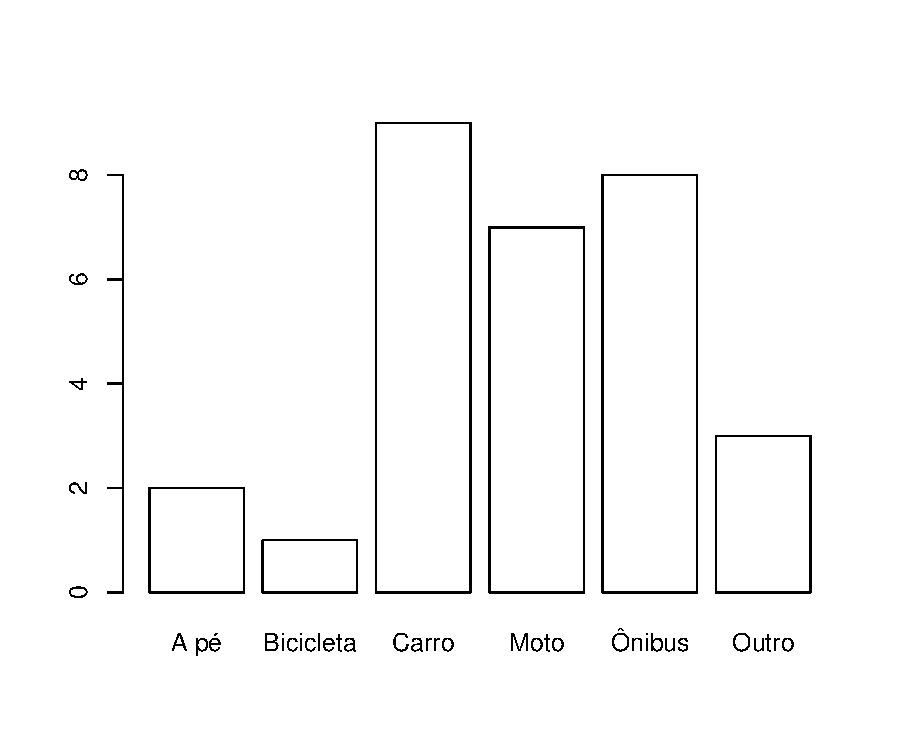
\includegraphics[width=0.9\linewidth]{exercicios-encontro1-solucao_files/figure-beamer/unnamed-chunk-4-1} \end{center}

\endColumns
\end{frame}

\begin{frame}{Exercício 3}
\phantomsection\label{exercuxedcio-3-3}
\beginAHalfColumn

\begin{longtable}[]{@{}lrr@{}}
\toprule\noalign{}
Respostas & \(f_a\) & \(f_r\) \\
\midrule\noalign{}
\endhead
Carro & 9 & 0.300 \\
Ônibus & 8 & 0.267 \\
Moto & 7 & 0.233 \\
Outro & 3 & 0.100 \\
A pé & 2 & 0.067 \\
Bicicleta & 1 & 0.033 \\
Total & 30 & 1.000 \\
\bottomrule\noalign{}
\end{longtable}

\endColumns
\beginAHalfColumn

\begin{center}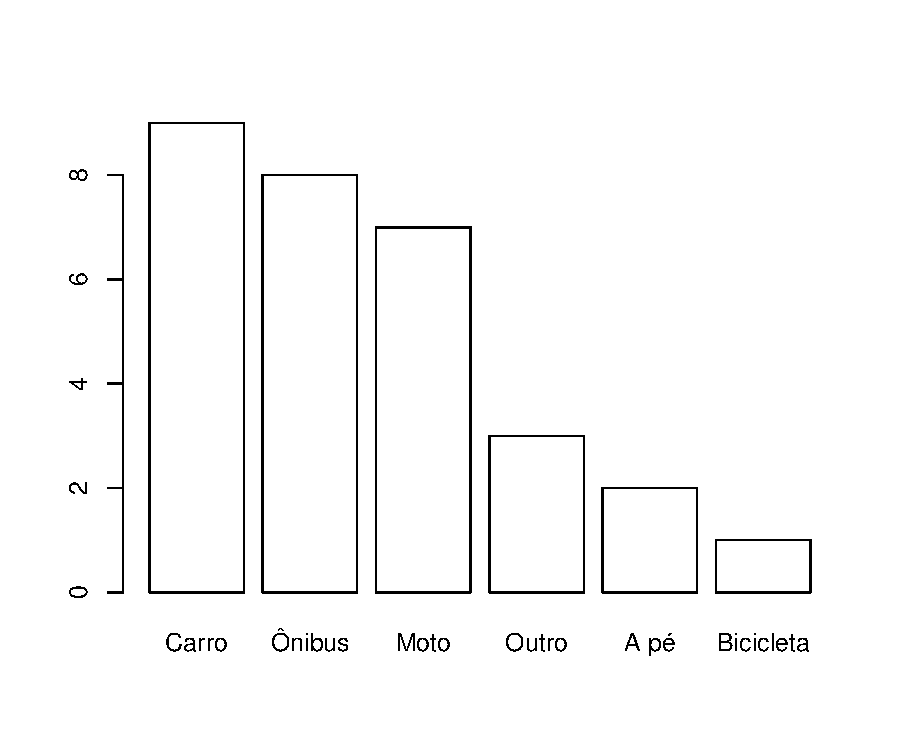
\includegraphics[width=0.9\linewidth]{exercicios-encontro1-solucao_files/figure-beamer/unnamed-chunk-6-1} \end{center}

\endColumns
\end{frame}

\begin{frame}{Exercício 3}
\phantomsection\label{exercuxedcio-3-4}
\beginAHalfColumn

\begin{longtable}[]{@{}lrr@{}}
\toprule\noalign{}
Respostas & \(f_a\) & \(f_r\) \\
\midrule\noalign{}
\endhead
Carro & 9 & 0.300 \\
Ônibus & 8 & 0.267 \\
Moto & 7 & 0.233 \\
Outro & 3 & 0.100 \\
A pé & 2 & 0.067 \\
Bicicleta & 1 & 0.033 \\
Total & 30 & 1.000 \\
\bottomrule\noalign{}
\end{longtable}

\endColumns
\beginAHalfColumn

\begin{center}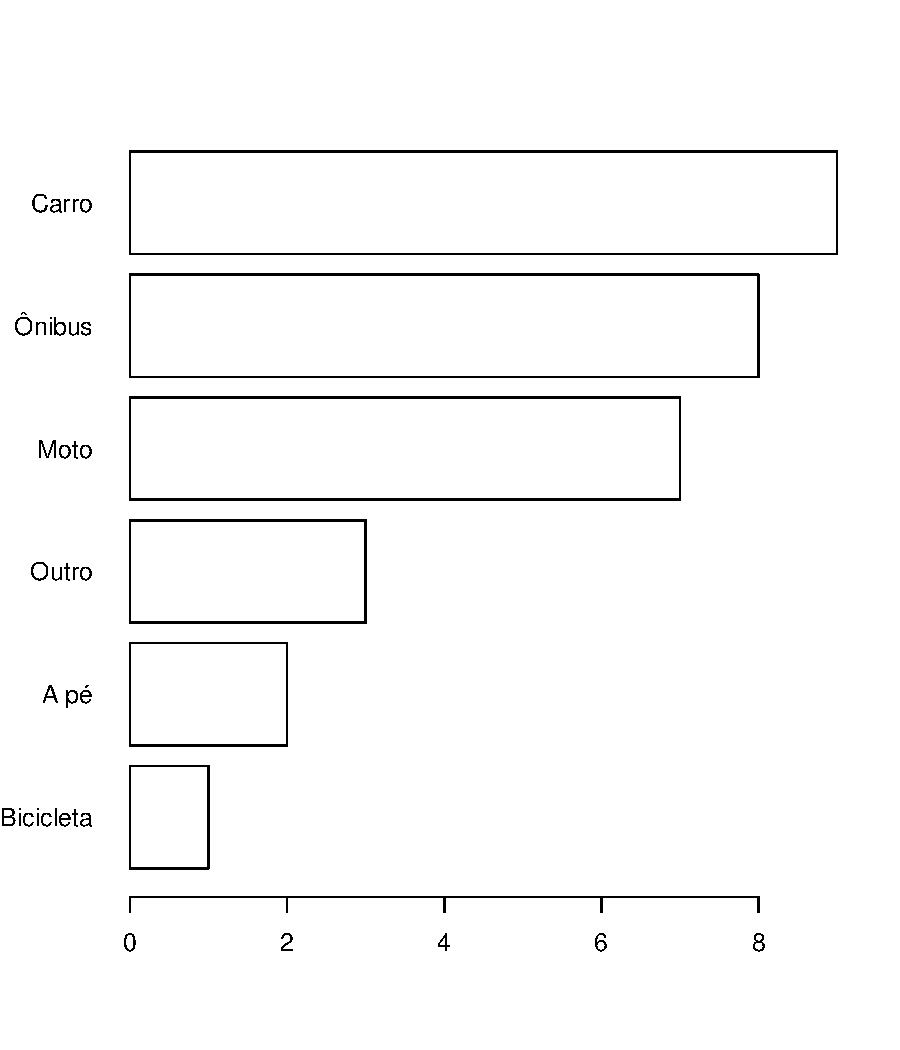
\includegraphics[width=0.9\linewidth]{exercicios-encontro1-solucao_files/figure-beamer/unnamed-chunk-8-1} \end{center}

\endColumns
\end{frame}

\section{Exercício 4}\label{exercuxedcio-4}

\begin{frame}{Exercício 4}
\phantomsection\label{exercuxedcio-4-1}
Diversas pesquisas de opinião fazem uso de um recurso chamado escala
Likert. A ideia é que afirmativas são apresentadas e o respondente
assinala o seu grau de concordância com cada afirmativa. Suponha que uma
pesquisa de opinião sobre a qualidade dos restaurantes universitários
está sendo conduzida e uma das afirmativas é ``os produtos utilizados
são de alta qualidade''. Um conjunto de respondentes tinha a
possibilidade de assinalar um de cinco pontos: discordo totalmente (DT);
discordo (D); indiferente (I); concordo (C) ou concordo totalmente (CT).

Considere o seguinte vetor de respostas:

\begin{longtable}[]{@{}llllllllllllllll@{}}
\toprule\noalign{}
\endhead
& C & D & I & C & DT & DT & C & CT & I & I & I & C & D & C & I \\
& CT & DT & C & I & C & I & I & CT & C & C & I & C & I & DT & C \\
\bottomrule\noalign{}
\end{longtable}

Construa uma tabela usando frequências absolutas, relativas (ou
percentuais) e acumuladas. Usando esta tabela esboce uma visualização
adequada.
\end{frame}

\begin{frame}{Exercício 4}
\phantomsection\label{exercuxedcio-4-2}
\beginAHalfColumn

\begin{longtable}[]{@{}lrrll@{}}
\toprule\noalign{}
Respostas & \(f_a\) & \(f_r\) & \(F_{a}\) & \(F_{r}\) \\
\midrule\noalign{}
\endhead
DT & 4 & 0.133 & 4 & 0.133 \\
D & 2 & 0.067 & 6 & 0.2 \\
I & 10 & 0.333 & 16 & 0.533 \\
C & 11 & 0.367 & 27 & 0.9 \\
CT & 3 & 0.100 & 30 & 1 \\
Total & 30 & 1.000 & & \\
\bottomrule\noalign{}
\end{longtable}

\endColumns
\beginAHalfColumn

\begin{center}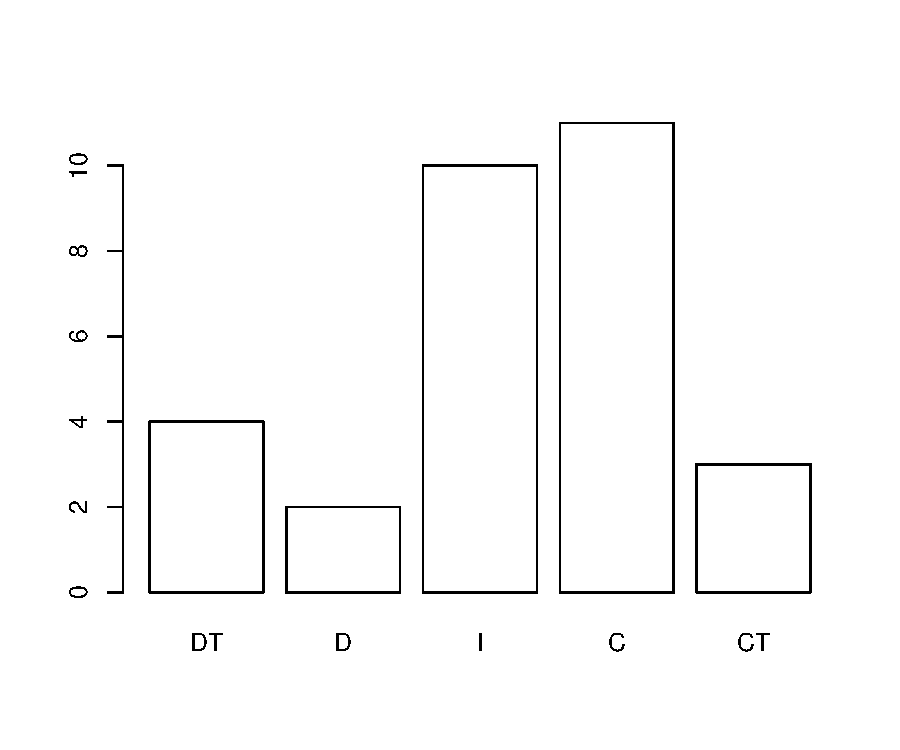
\includegraphics[width=0.9\linewidth]{exercicios-encontro1-solucao_files/figure-beamer/unnamed-chunk-11-1} \end{center}

\endColumns
\end{frame}

\begin{frame}{Exercício 4}
\phantomsection\label{exercuxedcio-4-3}
\beginAHalfColumn

\begin{longtable}[]{@{}lrrll@{}}
\toprule\noalign{}
Respostas & \(f_a\) & \(f_r\) & \(F_{a}\) & \(F_{r}\) \\
\midrule\noalign{}
\endhead
DT & 4 & 0.133 & 4 & 0.133 \\
D & 2 & 0.067 & 6 & 0.2 \\
I & 10 & 0.333 & 16 & 0.533 \\
C & 11 & 0.367 & 27 & 0.9 \\
CT & 3 & 0.100 & 30 & 1 \\
Total & 30 & 1.000 & & \\
\bottomrule\noalign{}
\end{longtable}

\endColumns
\beginAHalfColumn

\begin{center}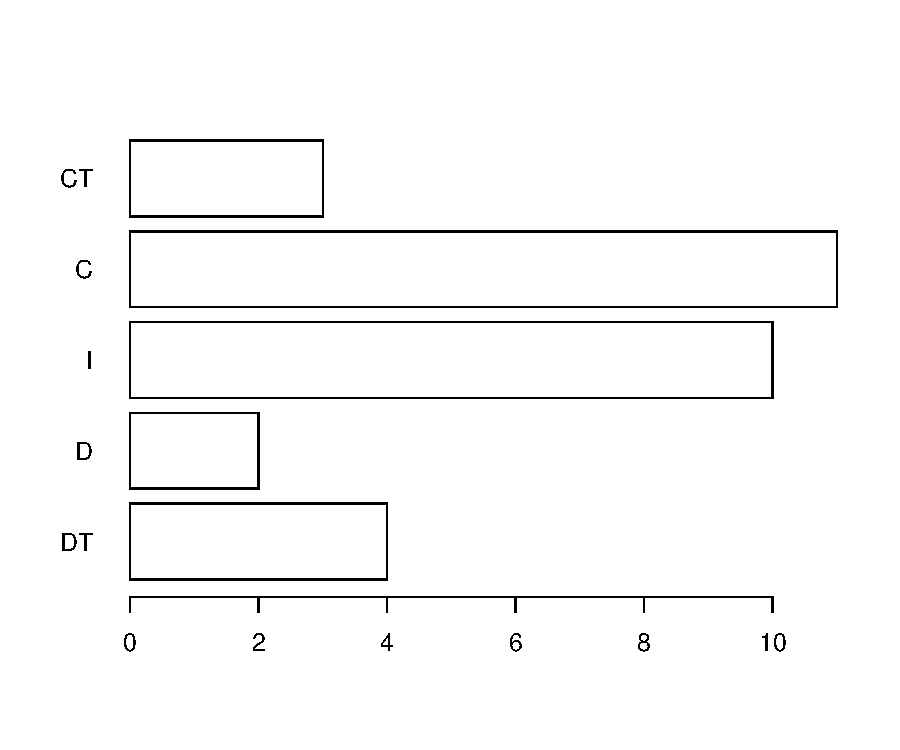
\includegraphics[width=0.9\linewidth]{exercicios-encontro1-solucao_files/figure-beamer/unnamed-chunk-13-1} \end{center}

\endColumns
\end{frame}

\section{Exercício 5}\label{exercuxedcio-5}

\begin{frame}{Exercício 5}
\phantomsection\label{exercuxedcio-5-1}
Uma empresa conduziu um estudo para avaliar a segurança de seus
funcionários. Um dos itens avaliados foi o número de acidentes sofrido
por cada funcionário em situações de trabalho. Os dados obtidos foram:

\begin{longtable}[]{@{}lllllllllll@{}}
\toprule\noalign{}
\endhead
& 0 & 0 & 1 & 8 & 0 & 8 & 7 & 1 & 1 & 0 \\
& 0 & 0 & 1 & 0 & 2 & 0 & 2 & 9 & 0 & 2 \\
& 7 & 0 & 1 & 0 & 0 & 0 & 0 & 0 & 6 & 0 \\
\bottomrule\noalign{}
\end{longtable}

Construa uma tabela usando frequências absolutas, relativas (ou
percentuais) e acumuladas. Usando esta tabela esboce uma visualização
adequada.
\end{frame}

\begin{frame}{Exercício 5}
\phantomsection\label{exercuxedcio-5-2}
\beginAHalfColumn

\begin{longtable}[]{@{}lrrll@{}}
\toprule\noalign{}
Respostas & \(f_a\) & \(f_r\) & \(F_{a}\) & \(F_{r}\) \\
\midrule\noalign{}
\endhead
0 & 16 & 0.533 & 16 & 0.533 \\
1 & 5 & 0.167 & 21 & 0.7 \\
2 & 3 & 0.100 & 24 & 0.8 \\
3 & 0 & 0.000 & 24 & 0.8 \\
4 & 0 & 0.000 & 24 & 0.8 \\
5 & 0 & 0.000 & 24 & 0.8 \\
6 & 1 & 0.033 & 25 & 0.833 \\
7 & 2 & 0.067 & 27 & 0.9 \\
8 & 2 & 0.067 & 29 & 0.967 \\
9 & 1 & 0.033 & 30 & 1 \\
10 & 0 & 0.000 & 30 & 1 \\
Total & 30 & 1.000 & & \\
\bottomrule\noalign{}
\end{longtable}

\endColumns
\beginAHalfColumn

\begin{center}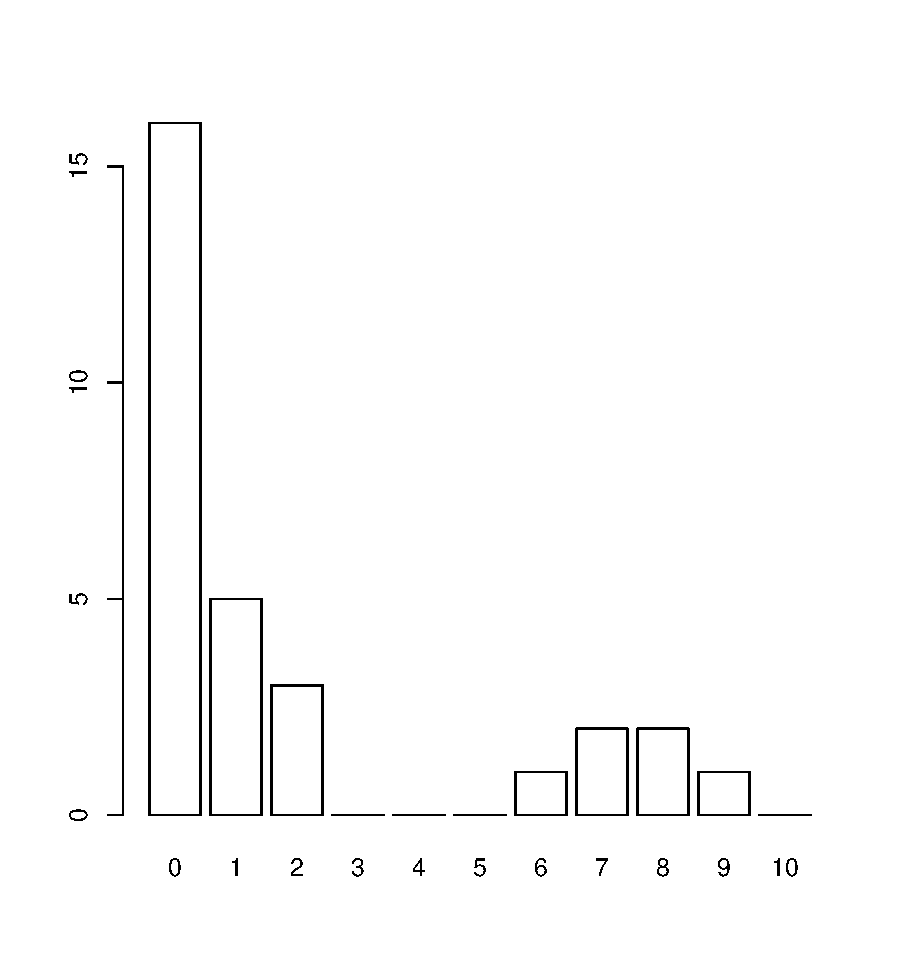
\includegraphics[width=0.9\linewidth]{exercicios-encontro1-solucao_files/figure-beamer/unnamed-chunk-16-1} \end{center}

\endColumns
\end{frame}

\section{Exercício 6}\label{exercuxedcio-6}

\begin{frame}{Exercício 6}
\phantomsection\label{exercuxedcio-6-1}
Existe interesse em estudar a altura de indivíduos de determinada
população. Para isso, uma amostra foi tomada e as alturas observadas (em
cm) foram:

\begin{longtable}[]{@{}lrrrrrrrrrr@{}}
\toprule\noalign{}
\endhead
& 161 & 172 & 186 & 159 & 169 & 171 & 177 & 168 & 190 & 169 \\
& 174 & 180 & 166 & 160 & 188 & 147 & 179 & 170 & 180 & 174 \\
& 191 & 158 & 186 & 190 & 170 & 145 & 175 & 164 & 178 & 173 \\
\bottomrule\noalign{}
\end{longtable}

Construa uma tabela usando com os dados agrupados em faixas de valores
partindo de 140 até 200 de 10 em 10. Use frequências absolutas,
relativas (ou percentuais) e acumuladas. Usando esta tabela esboce uma
visualização adequada.
\end{frame}

\begin{frame}{Exercício 6}
\phantomsection\label{exercuxedcio-6-2}
\beginAHalfColumn

\begin{longtable}[]{@{}lrrll@{}}
\toprule\noalign{}
Faixas & \(f_a\) & \(f_r\) & \(F_{a}\) & \(F_{r}\) \\
\midrule\noalign{}
\endhead
{[}140,150) & 2 & 0.067 & 2 & 0.067 \\
{[}150,160) & 2 & 0.067 & 4 & 0.133 \\
{[}160,170) & 7 & 0.233 & 11 & 0.367 \\
{[}170,180) & 11 & 0.367 & 22 & 0.733 \\
{[}180,190) & 5 & 0.167 & 27 & 0.9 \\
{[}190,200{]} & 3 & 0.100 & 30 & 1 \\
Total & 30 & 1.001 & & \\
\bottomrule\noalign{}
\end{longtable}

\endColumns
\beginAHalfColumn

\begin{center}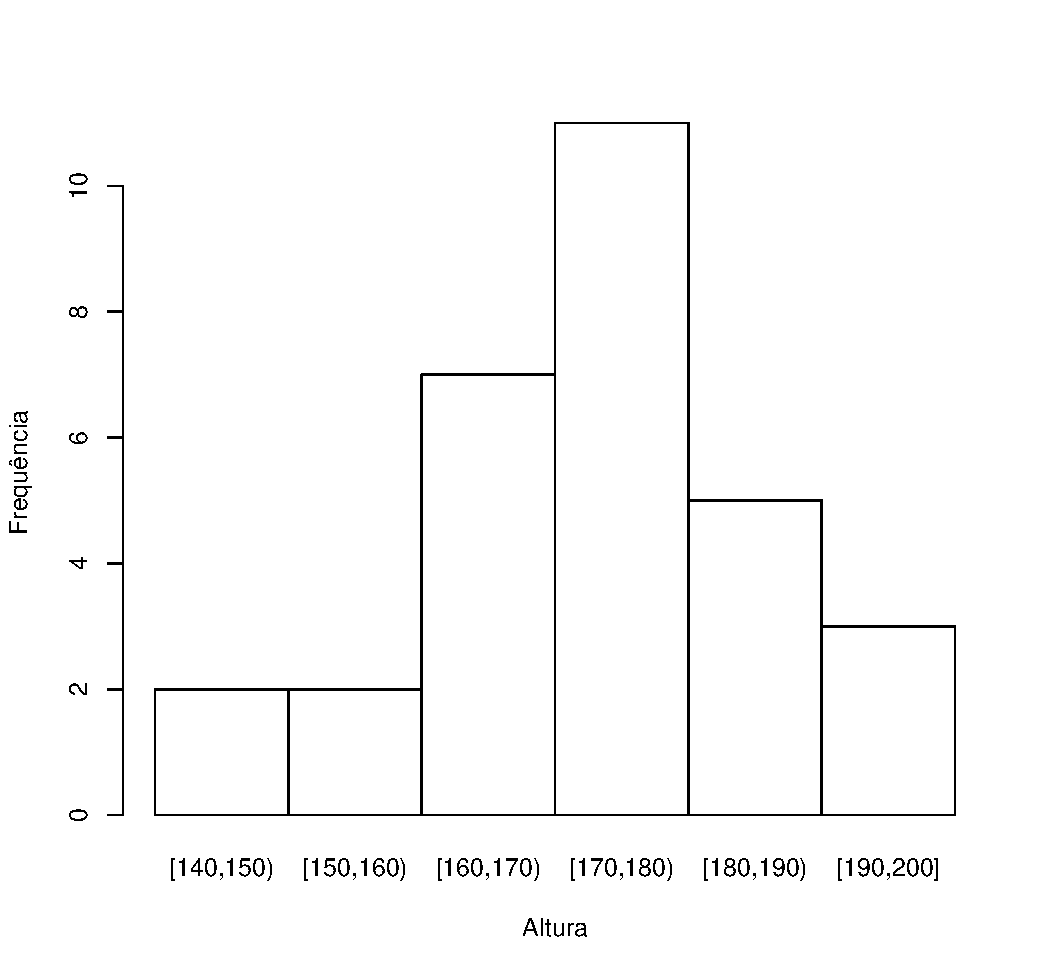
\includegraphics[width=0.9\linewidth]{exercicios-encontro1-solucao_files/figure-beamer/unnamed-chunk-19-1} \end{center}

\endColumns
\end{frame}

\end{document}
